\graphicspath{{../../S23_Representer_le_pave_et_le_cylindre/Images/}}

\themeG
\chapter{Représenter le pavé et le cylindre}
\label{S23}

\textcolor{ForestGreen}{\bf Compétences :}
   \begin{competences}
      \item Construire et mettre en relation des représentations des solides suivants : pavé droit et cylindre (perspective cavalière, patrons).
      \item Utiliser un logiciel de géométrie dynamique pour représenter des solides.
\end{competences}

\vfill

\begin{debat}{Débat : la perspective}
   La {\bf perspective cavalière} est un outil qui permet de représenter sur une feuille de papier des objets en volume sans point de fuite. \par
   Cette représentation était utilisée pour la conception des fortifications militaires. Le \og cavalier \fg{} était un promontoire de terre situé en arrière des fortifications et qui permettait de voir par-dessus la ligne des ouvrages de défense, et donc de voir les ouvrages des assaillants et ainsi d'anticiper leurs plans offensifs. D'autres perspectives sont utilisées notamment pour les arts : le perspective par {\bf point de fuite} et la {\bf perspective isométrique} par exemple.
   \tcblower
      {\psset{Decran=20,viewpoint=10 5 10,unit=0.45}
      \begin{pspicture}(-5,-4.5)(5,5)
         \psSolid[fcol=0 (red) 1 (Aquamarine) 2 (Bittersweet) 3 (ForestGreen) 4 (Goldenrod) 13 (GreenYellow) 40 (Mulberry), object=cube,mode=3]
      \end{pspicture}
      \begin{pspicture}(-5,-4)(5,5)
         \psSolid[fcol=0 (gray) 2 (Lavender) 3 (SkyBlue) 11 (LimeGreen) 12 (Brown) 23 (OliveGreen) 22 (Yellow) , object=cylindre,h=4,ngrid=4 10](0,0,-2)
      \end{pspicture}} 
\end{debat}

\hfill {\gray Vidéo : \href{https://www.youtube.com/watch?v=zCIxdOCQiZg}{\bf Comment dessiner des illusions d'optique 3D}, chaîne YouTube {\it Simple drawing tutorial}.}


%%% Approche %%%
\begin{Maquette}[Cours]{Theme={Activité d'approche},Couleur={SteelBlue}}

   \AAtitre{Patron à colorier}

      {\it Objectifs : résoudre un problème d'optimisation ; travailler sur les propriétés du patron du pavé droit.}

      \begin{AActivite}

         Avec le moins de couleurs possible, colorier le pavé droit dont voici un patron sachant que deux zones voisines ne doivent pas être de la même couleur.
         \begin{center}
            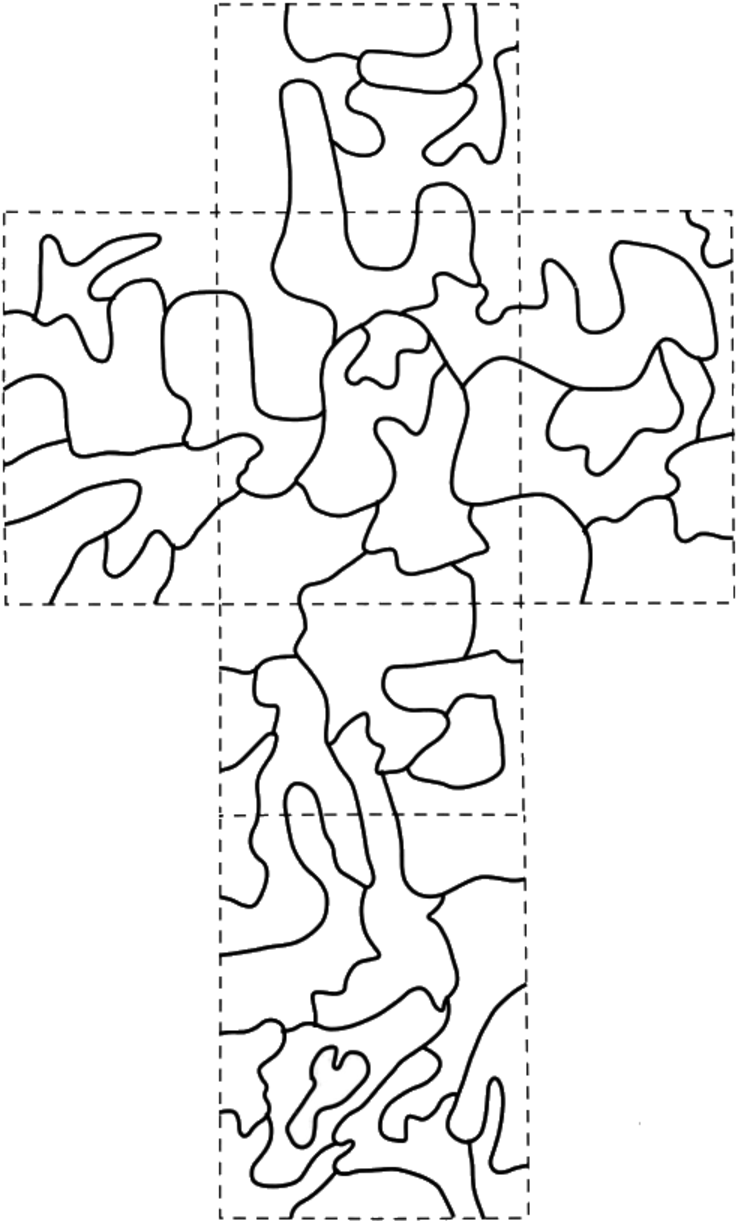
\includegraphics[width=12.5cm]{Pave_a_colorier}
         \end{center}

      \end{AActivite}

      \vfill\hfill{\it\footnotesize Source : \og Jeux 5 - Brochure APMEP n°117 \fg}.

\end{Maquette}


%%%Trace écrite %%%
\begin{Maquette}[Cours]{Theme={Trace écrite},Couleur={0.4[SteelBlue,Black]}}


   %%%1
   \section{Définitions}

      \begin{definition*}{}
         \begin{itemize}
            \item La représentation en \textbf{perspective cavalière} d'un solide de l'espace est une technique de dessin permettant de représenter un solide sur une surface à deux dimensions en respectant le parallélisme.
            \item Le \textbf{patron} d'un solide est une surface plane d'un seul tenant qui, par pliage, permet de reconstituer le solide sans recouvrement de ses faces.
            \item Si le solide n'est pas un polyèdre, on parle de {\bf développement}.
         \end{itemize}
      \end{definition*}

      Un patron se dessine en dépliant mentalement le solide.

      \begin{exemple*}{} 
         {\psset{fillstyle=solid,unit=0.3}
         \begin{pspicture}(-13,-4)(5,6)  
            \pspolygon[fillcolor=DodgerBlue](-5.38,-3.26)(-1.46,-3.74)(-2.88,-1.66)(-6.74,-1.04)
            \pspolygon[fillcolor=Yellow](-1.06,-1.36)(4.36,0.74)(3.94,-1.66)(-1.46,-3.74)
            \pspolygon[fillcolor=Crimson](-6.54,-0.46)(-5.24,3.82)(0.12,5.9)(-1.22,1.66)
            \pspolygon[fillcolor=DodgerBlue](4.48,1.22)(0.64,1.82)(0.12,-0.90)(4.36,0.74)
            \pspolygon[fillcolor=Yellow](0.12,-0.90)(-1.22,1.66)(-6.54,-0.46)(-6.27,-1.12)(-2.88,-1.66)(-2.55,-2.15)(-1.11,-1.68)(-1.06,-1.36)
            \pspolygon[fillcolor=Crimson](-1.46,-3.74)(-2.55,-2.15)(-1.11,-1.68)
         \end{pspicture}}
         {\psset{fillstyle=solid,unit=0.7}
         \begin{pspicture}(-4,0)(6,4.25)
            \psframe[fillcolor=Crimson](-1,1)(1,3.5)
            \psframe[fillcolor=Yellow](1,1)(2,3.5)
            \psframe[fillcolor=Crimson](2,1)(4,3.5)
            \psframe[fillcolor=Yellow](4,1)(5,3.5)
            \psframe[fillcolor=DodgerBlue](2,3.5)(4,4.5)
            \psframe[fillcolor=DodgerBlue](2,1)(4,0)
         \end{pspicture}}
      \end{exemple*}

      Le patron ou le développement d'un solide n'est pas unique, il dépend de la manière dont on le déplie.


   %%%2
   \section{Représentations graphiques}

      \begin{center}
         {\psset{unit=0.5} \small \hautab{1.5}
         \begin{tabular}{cC{7}|C{7}|}
            & \cellcolor{SteelBlue!50}{Pavé (droit)} & \cellcolor{SteelBlue!50}{Cylindre (de révolution)} \\
            \cellcolor{SteelBlue!50}{\rotatebox{90}{Perspective cavalière}}
            &
            \raisebox{0cm}{\psset{unit=1.2}
            \begin{pspicture}(0,-0.5)(5,5.5)
               \pspolygon(0,0)(4,0)(5,1)(5,4)(1,4)(0,3)
               \psline(0,3)(4,3)(4,0)
               \psline(4,3)(5,4)
               \psline[linestyle=dashed](0,0)(1,1)(5,1)
               \psline[linestyle=dashed](1,1)(1,4)
               \psdots[linecolor=Crimson](2,0)(3,1)(2,3)(3,4)
               \psdots[dotstyle=square*,linecolor=DodgerBlue](0,1.5)(4,1.5)(1,2.5)(5,2.5)
               \psdots[dotstyle=triangle*,linecolor=ForestGreen](0.5,0.5)(0.5,3.5)(4.5,0.5)(4.5,3.5)
            \end{pspicture}}
            &
            \raisebox{0cm}{\psset{unit=1.2}
            \begin{pspicture}(0,-0.5)(3.2,5.5)
               \psellipse(1.6,4)(1.6,0.5)
               \psellipticarc[linestyle=dashed](1.6,0)(1.6,0.5){0}{180}
               \psellipticarc(1.6,0)(1.6,0.5){180}{0}
               \psline(0,0)(0,4)  
               \psline(3.2,0)(3.2,4)
               \psdots[linecolor=Crimson](0,2)(3.2,2)
            \end{pspicture}} \\
            \cellcolor{SteelBlue!50}{\rotatebox{90}{\hskip1.8cm Patron ou développement}}
            &
            \raisebox{0cm}{\psset{unit=1.2}
            \begin{pspicture}(0,-1.75)(10,9)
               \pspolygon(2,0)(5,0)(5,2)(10,2)(10,6)(5,6)(5,8)(2,8)(2,6)(0,6)(0,2)(2,2)
               \psframe(2,2)(5,6)
               \psline(7,2)(7,6)
               \psdots[linecolor=Crimson](0,4)(2,4)(5,4)(7,4)(10,4)
               \psdots[dotstyle=square*,linecolor=DodgerBlue](3.5,0)(3.5,2)(3.5,6)(3.5,8)(8.5,2)(8.5,6)
               \psdots[dotstyle=triangle*,linecolor=ForestGreen](1,2)(1,6)(2,1)(2,7)(5,1)(5,7)(6,2)(6,6)
            \end{pspicture}}
            &
            \raisebox{0cm}{\psset{unit=1.2}
            \begin{pspicture}(0,-3.5)(10,8.5)
               \psframe(0,0)(10,4)
               \psline(0,0)(10,0)
               \psline(0,4)(10,4)
               \pscircle(2,5.6){1.6}
               \pscircle(6,-1.6){1.6}
               \psdots[linecolor=Crimson](0,2)(10,2)
            \end{pspicture}} \\
            \hline
         \end{tabular}}
      \end{center}
\end{Maquette}


%%% Exercices %%%
\begin{Maquette}[Fiche,CorrigeFin,Colonnes=2]{}

   \begin{exercice}[SLF] %1
      Terminer la représentation en perspective cavalière des trois pavés et du cylindre suivants :
      \begin{center}
         {\psset{unit=0.5}
         \begin{pspicture}(-1,-1)(30,6)
            \psgrid[subgriddiv=1,gridlabels=0pt,gridcolor=lightgray](-1,-1)(30,6)
            \psset{linewidth=0.7mm}
            \psline(0,2)(0,0)(2,0) % cube
            \psline[linestyle=dashed](0,0)(1,1)
            \psline(5,0)(5,4)(8,4)(10,5) % pavé 1
            \psline[linestyle=dashed](12,0)(13,2)(21,2) % pavé 2
            \psline[linestyle=dashed](13,2)(13,5)
            \psline(23,1)(23,4) % cylindre
            \psellipticarc(26,1)(3,0.5){180}{0}
         \end{pspicture}}
      \end{center}
   \end{exercice}
   
   \begin{Solution}
      {\psset{unit=0.4}
      \begin{pspicture}(-1,-1)(12,6.7)
         \psgrid[subgriddiv=1,gridlabels=0pt,gridcolor=lightgray](-1,-1)(12,6)
         \psset{linewidth=0.4mm}
         \psline(0,2)(0,0)(2,0) % cube
         \psline[linestyle=dashed](0,0)(1,1)
         \psline[linecolor=RoyalBlue](2,0)(3,1)(3,3)(1,3)(0,2)(2,2)(2,0)
         \psline[linecolor=RoyalBlue](2,2)(3,3)         
         \psline[linestyle=dashed,linecolor=RoyalBlue](3,1)(1,1)(1,3)
         \psline(5,0)(5,4)(8,4)(10,5) % pavé 1
         \psline[linecolor=RoyalBlue](5,0)(8,0)(10,1)(10,5)(7,5)(5,4)
         \psline[linecolor=RoyalBlue](8,0)(8,4)    
         \psline[linestyle=dashed,linecolor=RoyalBlue](5,0)(7,1)(10,1)
         \psline[linestyle=dashed,linecolor=RoyalBlue](7,1)(7,5)
      \end{pspicture} \par
      \begin{pspicture}(10,-1)(30,7)
         \psgrid[subgriddiv=1,gridlabels=0pt,gridcolor=lightgray](10,-1)(30,6)
         \psset{linewidth=0.4mm}
         \pspolygon[linecolor=RoyalBlue](12,0)(20,0)(21,2)(21,5)(13,5)(12,3) % pavé 2
         \psline[linecolor=RoyalBlue](12,3)(20,3)(21,5)
         \psline[linecolor=RoyalBlue](20,3)(20,0)         
         \psline[linestyle=dashed](12,0)(13,2)(21,2)
         \psline[linestyle=dashed](13,2)(13,5)
         \psline(23,1)(23,4) % cylindre
         \psline[linecolor=RoyalBlue](29,1)(29,4)
         \psellipticarc(26,1)(3,0.5){180}{0}
         \psellipticarc[linecolor=RoyalBlue,linestyle=dashed](26,1)(3,0.5){0}{180}
         \psellipse[linecolor=RoyalBlue](26,4)(3,0.5)
      \end{pspicture}}
   \end{Solution}
   
   
   \begin{exercice}[Dur] %2
      Tracer un maximum de patrons différents du cube (c'est-à-dire non superposables).
   \end{exercice}
   
   \begin{Solution}
      On obtient onze patrons différents : \par
      {\psset{unit=0.5,linecolor=RoyalBlue} 
      \begin{pspicture}(0,0)(4,4.5) %1
         \facer{0}{0} \facec{1}{0} \facec{1}{1} \facec{1}{2} \facec{1}{3} \facer{2}{0}
      \end{pspicture}
      \begin{pspicture}(0,0)(4,4.5) %2
         \facer{0}{0} \facec{1}{0} \facec{1}{1} \facec{1}{2} \facec{1}{3} \facer{2}{1}
      \end{pspicture}
      \begin{pspicture}(0,0)(4,4.5) %3
         \facer{0}{0} \facec{1}{0} \facec{1}{1} \facec{1}{2} \facec{1}{3} \facer{2}{2}
      \end{pspicture}
      \begin{pspicture}(0,0)(3.9,4.5) %4
         \facer{0}{0} \facec{1}{0} \facec{1}{1} \facec{1}{2} \facec{1}{3} \facer{2}{3}
      \end{pspicture} \medskip

      \begin{pspicture}(0,0)(4,4.5) %5
         \facer{0}{1} \facec{1}{0} \facec{1}{1} \facec{1}{2} \facec{1}{3} \facer{2}{1}
      \end{pspicture}
      \begin{pspicture}(0,0)(4,4.5) %6
         \facer{0}{1} \facec{1}{0} \facec{1}{1} \facec{1}{2} \facec{1}{3} \facer{2}{2}
      \end{pspicture}
      \begin{pspicture}(0,0)(4,3.5) %11
         \facec{0}{0} \facec{1}{0} \face{1}{1} \face{2}{1} \face{2}{2} \face{3}{2}
      \end{pspicture} \medskip

      \begin{pspicture}(0,-2)(4,4.5) %7
         \facec{1}{1} \facec{1}{2} \facec{1}{3} \face{2}{0} \face{2}{1} \facer{0}{3}
      \end{pspicture}
      \begin{pspicture}(0,-2)(4,4.5) %8
         \facec{1}{1} \facec{1}{2} \facec{1}{3} \face{2}{0} \face{2}{1} \facer{0}{2}
      \end{pspicture}
      \begin{pspicture}(0,-2)(3,4.5) %9
         \facec{1}{1} \facec{1}{2} \facec{1}{3} \face{2}{0} \face{2}{1} \facer{0}{1}
      \end{pspicture}
      \begin{pspicture}(0,-2)(4,4) %10
         \facec{1}{1} \facec{1}{2} \facec{1}{3} \face{2}{0} \face{2}{1} \facer{2}{-1}
      \end{pspicture}}
   \end{Solution}
   
   
   \begin{exercice}[Dur] %3
      Construire en vraie grandeur un patron des solides suivants : 
      \begin{enumerate}
         \item Pavé droit de mesures \Lg{5} ; \Lg{4} et \Lg{2}.
         \item Cylindre de révolution de hauteur \Lg{8} dont le diamètre de la base vaut \Lg{2}.
         \item Cylindre de révolution de hauteur \Lg{2} dont le rayon de la base vaut \Lg{2,5}.
      \end{enumerate}
   \end{exercice}
   
   \begin{Solution}
      Un carreau représente un carré de \Lg{1} de côté.
      \begin{enumerate}
         \item Patron du pavé de mesures \Lg{5}, \Lg{4} et \Lg{2}. \par
            {\psset{unit=0.5}
            \begin{pspicture}(0,0)(14,11.5)
               \psset{linecolor=RoyalBlue}
               \psgrid[subgriddiv=1,gridlabels=0pt,gridcolor=lightgray](0,0)(14,11)
               \psline(3,1)(3,3)(1,3)(1,8)(3,8)(3,10)(7,10)(7,8)(13,8)(13,3)(7,3)(7,1)(3,1)
               \psframe(3,3)(7,8)
               \psline(9,3)(9,8)
            \end{pspicture}}
         \item Développement du cylindre de hauteur \Lg{8} de diamètre \Lg{2} : le périmètre du disque vaut \par \smallskip
            $2\times\pi\times\dfrac{\Lg{2}}{2} \approx\Lg{6,28}$. \par
            {\psset{unit=0.5}
            \begin{pspicture}(-1,-1.5)(13,7.5)
               \psgrid[subgriddiv=1,gridlabels=0pt,gridcolor=lightgray](-1,-1)(13,7)
               \psset{linecolor=RoyalBlue}
               \psframe(2,0)(10,6.28)
               \pscircle(1,3){1}
               \pscircle(11,3){1}
               \psdots(1,3)(11,3)
            \end{pspicture}}
         \item Développement du cylindre de hauteur \Lg{2} de rayon \Lg{2,5} : le périmètre du disque vaut \par
            $2\times\pi\times\Lg{2,5} \approx\Lg{15,71}$. \par
           {\psset{unit=0.41}
           \begin{pspicture}(-1,-1)(16,14)
              \psgrid[subgriddiv=1,gridlabels=0pt,gridcolor=lightgray](-1,-1)(16,13)
              \psset{linecolor=RoyalBlue}
              \psframe(0,5)(15.7,7)
              \pscircle(5,2.5){2.5}
              \pscircle(8,9.5){2.5}
              \psdots(5,2.5)(8,9.5)
            \end{pspicture}}
      \end{enumerate}
   \end{Solution}
   
   
   \begin{exercice}[SLF] %4
      Parmi tous ces patrons, quels sont ceux qui permettent de construire un pavé ?
      \begin{center}
         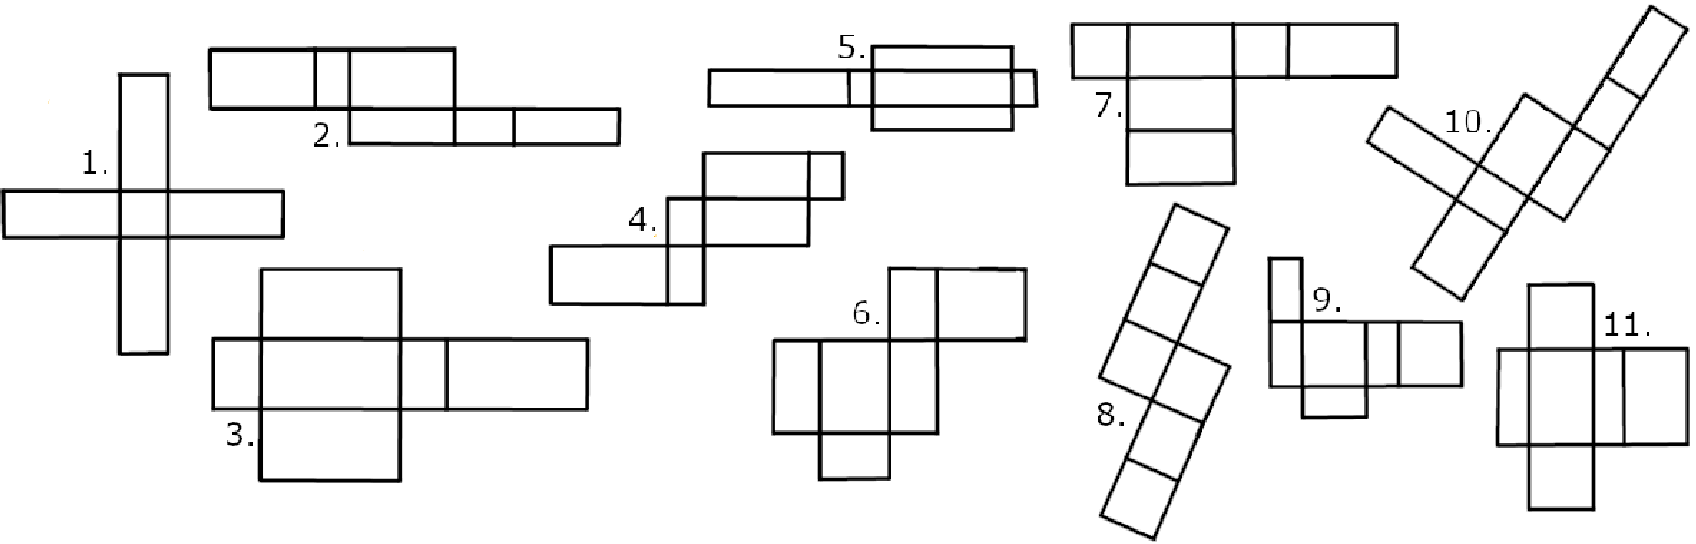
\includegraphics[width=16cm]{patrons_paves}
      \end{center}
   \end{exercice}
   
   \begin{Solution}
      \begin{itemize}
         \item Les figures \cor{2, 5, 6, 8; 9} sont des patrons de pavés.
         \item Les figures 1 et 10 n'ont pas le bon nombre de faces (5 et 7).
         \item Les figures 3, 4 et 11 possèdent des arêtes qui ne se correspondent pas.
         \item La figure 7 a deux faces qui se superposent.
      \end{itemize}
   \end{Solution}
   
   \begin{exercice}[SLF] %5
      Parmi tous ces développements, quels sont ceux qui permettent de construire un cylindre ? \smallskip
      \begin{center}
         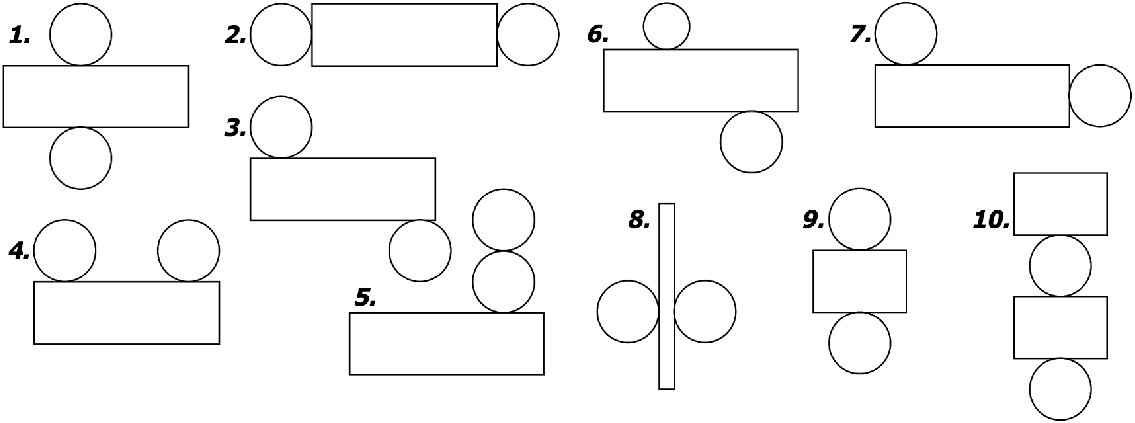
\includegraphics[width=16cm]{patrons_cylindres}
      \end{center}
   \end{exercice}
   
   \begin{Solution}
      \begin{itemize}
         \item Les figures \cor{1, 3, 8 et 10 sont les développements de cylindres} (la figure 10 est un cas particulier avec une surface divisée en deux parties).
         \item Les figures 2 et 9 possèdent un rectangle trop court par rapport au périmètre du disque.
         \item Les figures 4, 5 et 7 ont un disque mal placé.
         \item La figure 6 possède un disque trop petit.
      \end{itemize}
   \end{Solution}

\end{Maquette}


%%% Récré %%%
\begin{Maquette}[Cours]{Theme={Activité récréative},Couleur={IndianRed}}
    
   \ARtitre{Des dessins magiques}

      {\psset{unit=0.7}
      \begin{pspicture*}(-1,-3)(24.5,30)
         \multido{\i=-17+1}{48}{\rput(\i;90){\multido{\n=-1+1}{30}{\psdot[linewidth=0.05mm,linecolor=gray](\n;30)}}} % quadrillage
         \cubiso{1.732}{1}
         \cubiso{5.196}{1}
         \cubiso{8.66}{1}
         \cubiso{3.464}{4}
         \cubiso{6.928}{4}
         \cubiso{5.196}{7}
         \rput(0,18){ % trident
            \psline(0,0)(19;30)(23.383,5.5)(8;-30)
            \psline(0,-2)(16.454,7.5)(19.919,5.5)(3.464,-4)
            \psline(23.383,5.5)(23.383,3.5)(6.928,-6)
            \psline(16.454,7.5)(16.454,5.5)(18.187,4.5)
            \psline(16.454,5.5)(3.464,-2)
            \psellipse(0,-1)(0.4,0.98)
            \psellipse(3.464,-3)(0.4,0.98)
            \psellipse(6.928,-5)(0.4,0.98)}
         \psset{fillstyle=solid,fillcolor=ForestGreen}
         \rput(3.464,-2){\pspolygon(2;90)(2;30)(4;30)(3.464;60)}
         \rput(6.928,-2){\pspolygon(2;90)(2;30)(4;30)(3.464;60)}
         \psset{fillcolor=Crimson}
         \rput(8.66,7){\pspolygon(0,0)(2;90)(2;30)(2;-30)}
         \rput(10.393,4){\pspolygon(0,0)(2;90)(2;30)(2;-30)}
         \psset{fillcolor=DodgerBlue}
         \rput(0,4){\pspolygon(2;-30)(3.464;0)(4;30)(2;30)}
         \rput(1.732,7){\pspolygon(2;-30)(3.464;0)(4;30)(2;30)}
         \rput(17;30){ %triangle impossible
            \pspolygon[fillcolor=DodgerBlue](0,0)(8;-30)(7.794,-3.5)(1.732,0)(6.062,2.5)(6.062,3.5)(7;30)
            \pspolygon[fillcolor=DarkViolet](0,0)(7;30)(6.062,-1.5)(6.928,-2)(6.928,5)(1;90)
            \pspolygon[fillcolor=DarkOrange](1.732,0)(7.794,-3.5)(7.794,4.5)(6.928,5)(6.928,-2)(2.598,0.5)}
         \psframe[fillstyle=solid,fillcolor=white,linecolor=white](0,25)(6,27.5)
         \rput(3,26.6){Reproduire ces dessins}
         \rput(3,25.8){sur du papier pointé}
      \end{pspicture*}} \vskip5mm

   
   \pagebreak
   
   {\psset{unit=0.7}
   \begin{pspicture*}(-1,-3)(24.5,34)
      \multido{\i=-20+1}{55}{\rput(\i;90){\multido{\n=-1+1}{30}{\psdot[linewidth=0.05mm,linecolor=gray](\n;30)}}}
   \end{pspicture*}}

\end{Maquette}